\section{Vectores Aleatorios}

\begin{ejercicio}
    Asociadas al experimento aleatorio de lanzar un dado y una moneda no cargados, se define la variable $X$ como el valor del dado y la variable $Y$, que toma el valor 0 si sale cara en la moneda, y 1 si sale cruz. Calcular la función masa de probabilidad y la función de distribución del vector aleatorio $(X,Y)$.\\

    Calculemos los recorreidos de $X$ e $Y$:
    \begin{align*}
        E_X &= \{1, 2, 3, 4, 5, 6\}, \\
        E_Y &= \{0, 1\}.
    \end{align*}

    Por tanto, tenemos que:
    \begin{equation*}
        E_{(X,Y)} = \{(1,0), (1,1), (2,0), (2,1), (3,0), (3,1), (4,0), (4,1), (5,0), (5,1), (6,0), (6,1)\}.
    \end{equation*}

    La función masa de probabilidad es:
    \Func{P_{(X,Y)}}{E_{(X,Y)}}{[0,1]}{(x,y)}{\nicefrac{1}{12}}

    Para poder calcular la función de distribución, primero representamos los puntos del espacio muestral en el plano cartesiano:
    \begin{figure}[H]
        \centering
        \begin{tikzpicture}
            \begin{axis}[
                axis lines = center,
                xlabel = $X$,
                ylabel = $Y$,
                xmin = 0, xmax = 7,
                ymin = -1, ymax = 2,
                xtick = {1,2,3,4,5,6},
                ytick = {0,1},
                yticklabels = {0, 1},
                yticklabel style = {xshift=-1.5ex},
                xticklabel style = {xshift=-1.5ex},
            ]
                \addplot[only marks] coordinates {
                    (1,0) (1,1) (2,0) (2,1) (3,0) (3,1) (4,0) (4,1) (5,0) (5,1) (6,0) (6,1)
                };

                % Líneas verticales
                \foreach \x in {1,2,3,4,5,6} {
                    \addplot[dashed] coordinates {(\x, -1) (\x, 2)};
                }

                % Líneas horizontales
                \foreach \y in {1} {
                    \addplot[dashed] coordinates {(0, \y) (7, \y)};
                }
            \end{axis}
        \end{tikzpicture}
    \end{figure}

    La función de distribución es:
    \begin{equation*}
        F_{(X,Y)}(x,y) = \begin{cases}
            0, & x<1 \text{ o } y<0, \\
            \nicefrac{1}{12}, & x\in \left[1,2\right[ \text{ y } y\in \left[0,1\right[, \\
            \nicefrac{2}{12}, & x\in \left[2,3\right[ \text{ y } y\in \left[0,1\right[ \quad \text{o} \quad x\in \left[1,2\right[ \text{ y } y\geq 1, \\
            \nicefrac{3}{12}, & x\in \left[3,4\right[ \text{ y } y\in \left[0,1\right[, \\
            \nicefrac{4}{12}, & x\in \left[4,5\right[ \text{ y } y\in \left[0,1\right[ \quad \text{o} \quad x\in \left[2,3\right[ \text{ y } y\geq 1, \\
            \nicefrac{5}{12}, & x\in \left[5,6\right[ \text{ y } y\in \left[0,1\right[ \quad \text{o} \quad x\in \left[3,4\right[ \text{ y } y\geq 1, \\
            \nicefrac{6}{12}, & x\geq 6 \text{ y } y\in \left[0,1\right[ \quad \text{o} \quad x\in \left[3,4\right[ \text{ y } y\geq 1, \\
            \nicefrac{8}{12}, & x\in \left[4,5\right[ \text{ y } y\geq 1, \\
            \nicefrac{10}{12}, & x\in \left[5,6\right[ \text{ y } y\geq 1, \\
            1, & x\geq 6 \text{ y } y\geq 1.
        \end{cases}
    \end{equation*}
\end{ejercicio}

\begin{ejercicio}
    El número de automóviles utilitarios, $X$, y el de automóviles de lujo, $Y$, que poseen las familias de una población se distribuye de acuerdo a las siguientes probabilidades:
    \begin{table}[H]
        \centering
        \begin{tabular}{c|ccc}
            $X\backslash Y$ & 0 & 1 & 2 \\
            \hline
            0 & \nicefrac{1}{3} & \nicefrac{1}{12} & \nicefrac{1}{24} \\
            1 & \nicefrac{1}{6} & \nicefrac{1}{24} & \nicefrac{1}{48} \\
            2 & \nicefrac{5}{22} & \nicefrac{5}{88} & \nicefrac{5}{176} \\
        \end{tabular}
    \end{table}
    Calcular la función de distribución del vector $(X,Y)$ en los puntos $(0,0)$; $(0,2)$; $(1,1)$ y $(2,1)$, y la probabilidad de que una familia tenga tres o más automóviles.\\

    Para calcular la función de distribución en los puntos $(0,0)$; $(0,2)$; $(1,1)$ y $(2,1)$, representamos antes los elementos de $E_{(X,Y)}$ en el plano cartesiano:
    \begin{figure}[H]
        \centering
        \begin{tikzpicture}[scale=0.8]
            \begin{axis}[
                axis lines = center,
                xlabel = $X$,
                ylabel = $Y$,
                xmin = -1, xmax = 3,
                ymin = -1, ymax = 3,
                xtick = {0,1,2},
                ytick = {0,1,2},
                yticklabels = {0, 1, 2},
                yticklabel style = {yshift=-1.5ex},
                xticklabel style = {xshift=-1.5ex},
            ]
                \addplot[only marks] coordinates {
                    (0,0) (0,1) (0,2) (1,0) (1,1) (1,2) (2,0) (2,1) (2,2)
                };

                % Líneas verticales
                \foreach \x in {1,2} {
                    \addplot[dashed] coordinates {(\x, -1) (\x, 3)};
                }

                % Líneas horizontales
                \foreach \y in {1,2} {
                    \addplot[dashed] coordinates {(-1, \y) (3, \y)};
                }
            \end{axis}
        \end{tikzpicture}
    \end{figure}

    La función de distribución en los puntos $(0,0)$; $(0,2)$; $(1,1)$ y $(2,1)$ es:
    \begin{align*}
        F_{(X,Y)}(0,0) &= P_{(X,Y)}(0,0) = \nicefrac{1}{3}, \\
        F_{(X,Y)}(0,2) &= P_{(X,Y)}(0,0) + P_{(X,Y)}(0,1) + P_{(X,Y)}(0,2) = \nicefrac{1}{3} + \nicefrac{1}{12} + \nicefrac{1}{24} = \nicefrac{11}{24}, \\
        F_{(X,Y)}(1,1) &= P_{(X,Y)}(0,0) + P_{(X,Y)}(0,1) + P_{(X,Y)}(1,0) + P_{(X,Y)}(1,1) = \nicefrac{1}{3} + \nicefrac{1}{12} + \nicefrac{1}{6} + \nicefrac{1}{24} = \nicefrac{5}{8}, \\
        F_{(X,Y)}(2,1) &= F_{(X,Y)}(1,1) + P_{(X,Y)}(2,0) + P_{(X,Y)}(2,1) = \nicefrac{5}{8} + \nicefrac{5}{22} + \nicefrac{5}{88} = \nicefrac{10}{11}.
    \end{align*}

    La probabilidad de que una familia tenga tres o más automóviles es:
    \begin{equation*}
        P[X+Y \geq 3] = P_{(X,Y)}(1,2) + P_{(X,Y)}(2,1) + P_{(X,Y)}(2,2) = \nicefrac{1}{48} + \nicefrac{5}{88} + \nicefrac{5}{176} = \nicefrac{7}{66}.
    \end{equation*}
    % // TODO: Por qué
\end{ejercicio}

\begin{ejercicio}
    La función de densidad del vector aleatorio $(X,Y)$, donde $X$ denota los Kg. de naranjas, e $Y$ los Kg. de manzanas vendidos al día en una frutería está dada por:
    \[
        f(x, y) = \frac{1}{400}; \quad 0 < x < 20; \quad 0 < y < 20.
    \]
    siendo esta nula en caso contrario.
    Determinar la función de distribución de $(X,Y)$ y la probabilidad de que en un día se vendan entre naranjas y manzanas, menos de 20 kilogramos.\\

    Representamos los puntos de discontinuidad de la función de densidad en el plano cartesiano:
    \begin{figure}[H]
        \centering
        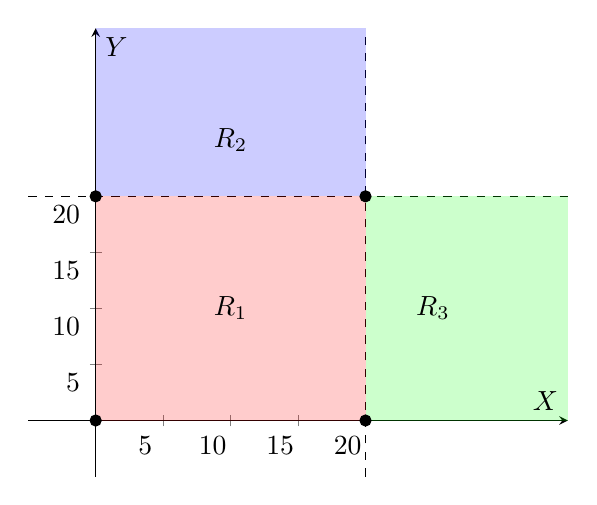
\begin{tikzpicture}
            \begin{axis}[
                axis lines = center,
                xlabel = $X$,
                ylabel = $Y$,
                xmin = -5, xmax = 35,
                ymin = -5, ymax = 35,
                xtick = {0,5,10,15,20},
                ytick = {0,5,10,15,20},
                yticklabel style = {yshift=-1.5ex},
                xticklabel style = {xshift=-1.5ex},
            ]
                \addplot[only marks] coordinates {
                    (0,0) (20,0) (0,20) (20,20)
                };

                % Líneas verticales
                \foreach \x in {20} {
                    \addplot[dashed] coordinates {(\x, -5) (\x, 35)};
                }

                % Líneas horizontales
                \foreach \y in {20} {
                    \addplot[dashed] coordinates {(-5, \y) (35, \y)};
                }                

                % Coloreamos cada una de las zonas
                \fill[red, opacity=0.2] (0,0) -- (20,0) -- (20,20) -- (0,20) -- cycle;
                \fill[blue, opacity=0.2] (0,20) -- (0,35) -- (20,35) -- (20,20) -- cycle;
                \fill[green, opacity=0.2] (20,0) -- (20,20) -- (35,20) -- (35,0) -- cycle;

                % Damos nombres a cada una de las zonas formadas
                \node at (10,10) {$R_1$};
                \node at (10,25) {$R_2$};
                \node at (25,10) {$R_3$};
            \end{axis}
        \end{tikzpicture}
    \end{figure}

    La función de distribución es:
    \begin{equation*}
        F_{(X,Y)}(x, y) = \int_{-\infty}^x \int_{-\infty}^y f(u, v) \, du \, dv
    \end{equation*}

    Estudiemos cada región por separado:
    \begin{itemize}
        \item \ul{Para $x\leq 0$ o $y\leq 0$}:
        
        Tenemos que $f(u, v) = 0$ para $u\leq x$ o $v\leq y$, por lo que:
        \begin{equation*}
            F_{(X,Y)}(x, y) = \int_{-\infty}^x \int_{-\infty}^y f(u, v) \, du \, dv =
            \int_{-\infty}^x \int_{-\infty}^y 0 \, du \, dv = 0.
        \end{equation*}

        \item \ul{Para $0 < x < 20$ y $0 < y < 20$} (región $R_1$):
        
        Tenemos que:
        \begin{equation*}
            F_{(X,Y)}(x, y) = \int_{-\infty}^x \int_{-\infty}^y f(u, v) \, du \, dv =
            \int_{0}^x \int_{0}^y \frac{1}{400} \, du \, dv = \frac{xy}{400}.
        \end{equation*}

        \item \ul{Para $0 < x < 20$ y $y \geq 20$} (región $R_2$):
        
        Tenemos que:
        \begin{equation*}
            F_{(X,Y)}(x, y) = \int_{-\infty}^x \int_{-\infty}^y f(u, v) \, du \, dv =
            \int_{0}^x \int_{0}^{20} \frac{1}{400} \, du \, dv = \frac{20x}{400} = \frac{x}{20}.
        \end{equation*}

        \item \ul{Para $x \geq 20$ y $0 < y < 20$} (región $R_3$):
        
        Tenemos que:
        \begin{equation*}
            F_{(X,Y)}(x, y) = \int_{-\infty}^x \int_{-\infty}^y f(u, v) \, du \, dv =
            \int_{0}^{20} \int_{0}^y \frac{1}{400} \, du \, dv = \frac{20y}{400} = \frac{y}{20}.
        \end{equation*}

        \item \ul{Para $x \geq 20$ y $y \geq 20$}:
        
        Tenemos que:
        \begin{equation*}
            F_{(X,Y)}(x, y) = \int_{-\infty}^x \int_{-\infty}^y f(u, v) \, du \, dv =
            \int_{0}^{20} \int_{0}^{20} \frac{1}{400} \, du \, dv = \frac{400}{400} = 1.
        \end{equation*}
    \end{itemize}

    Por tanto, la función de distribución es:
    \begin{equation*}
        F_{(X,Y)}(x, y) = \begin{cases}
            0, & x\leq 0 \text{ o } y\leq 0, \\
            \frac{xy}{400}, & 0 < x < 20 \text{ y } 0 < y < 20, \\
            \frac{x}{20}, & 0 < x < 20 \text{ y } y\geq 20, \\
            \frac{y}{20}, & x\geq 20 \text{ y } 0 < y < 20, \\
            1, & x\geq 20 \text{ y } y\geq 20.
        \end{cases}
    \end{equation*}

    Buscamos ahora la probabilidad de que en un día se vendan entre naranjas y manzanas, menos de 20 kilogramos. Para ello, buscamos la región del plano que cumple con la condición $X+Y < 20$. Tras representar la recta $y=20-x$,
    nos quedaremos con la región que queda por debajo de esta recta:
    \begin{figure}[H]
        \centering
        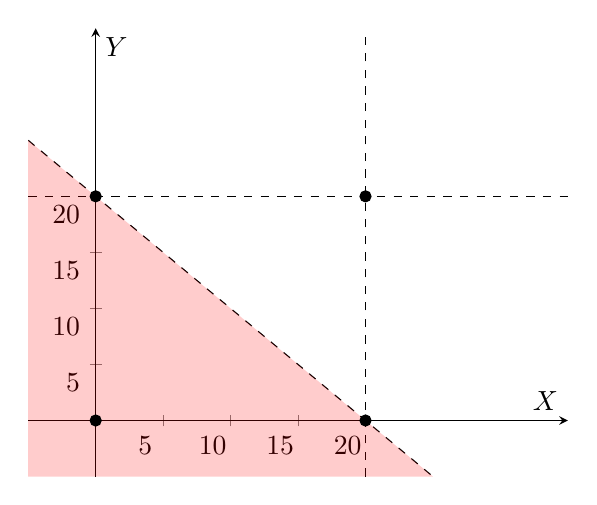
\begin{tikzpicture}
            \begin{axis}[
                axis lines = center,
                xlabel = $X$,
                ylabel = $Y$,
                xmin = -5, xmax = 35,
                ymin = -5, ymax = 35,
                xtick = {0,5,10,15,20},
                ytick = {0,5,10,15,20},
                yticklabel style = {yshift=-1.5ex},
                xticklabel style = {xshift=-1.5ex},
            ]
                \addplot[only marks] coordinates {
                    (0,0) (20,0) (0,20) (20,20)
                };

                % Líneas verticales
                \foreach \x in {20} {
                    \addplot[dashed] coordinates {(\x, -5) (\x, 35)};
                }

                % Líneas horizontales
                \foreach \y in {20} {
                    \addplot[dashed] coordinates {(-5, \y) (35, \y)};
                }

                % Representamos la recta y=20-x
                \addplot[domain=-5:35, samples=2, dashed] {20-x};

                % Coloreamos la región entre el (-5, 25), (25, -5) y (-5,-5)
                \fill[red, opacity=0.2] (-5,25) -- (25,-5) -- (-5,-5) -- cycle;
            \end{axis}
        \end{tikzpicture}
    \end{figure}

    Por tanto, tenemos que $P[X+Y < 20]$ es la integral de la función de densidad en la región coloreada, $R=\{(x,y)\in \mathbb{R}^2; x+y<20\}$:
    \begin{align*}
        P[X+Y < 20] &= \int_{-\infty}^{+\infty} \int_{-\infty}^{20-x} f(x, y) \, dy \, dx = \int_{0}^{20} \int_{0}^{20-x} \frac{1}{400} \, dy \, dx =\\&= \int_{0}^{20} \frac{20-x}{400} \, dx = \frac{1}{400}\left[20x-\frac{x^2}{2}\right]_0^{20} = \frac{1}{400}\left[400-200\right] = \frac{1}{2}.
    \end{align*}
\end{ejercicio}

\begin{ejercicio}
    La renta, $X$, y el consumo, $Y$, de los habitantes de una población, tienen por funciones de densidad
    \[
        f_X(x) = 2-2x; \quad 0 < x < 1; \quad f_{Y\mid X} (y\mid x) = \frac{1}{x}; \quad 0 < y < x.
    \]
    Determinar la función de densidad conjunta del vector aleatorio $(X,Y)$ y la probabilidad de que el consumo sea inferior a la mitad de la renta.\\

    Tenemos que, para $R=\{(x,y)\in \mathbb{R}^2; 0<x<1, 0<y<x\}$, la función de densidad conjunta es:
    \begin{equation*}
        f_{Y\mid X} (y\mid x) = \dfrac{f_{(X,Y)}(x, y)}{f_X(x)} \Longrightarrow f_{(X,Y)}(x, y) = f_X(x) \cdot f_{Y\mid X} (y\mid x) = (2-2x) \cdot \dfrac{1}{x} = \dfrac{2-2x}{x}.
    \end{equation*}

    Tenemos ahora que:
    \begin{align*}
        P[Y < \nicefrac{X}{2}] &= \int_{-\infty}^{+\infty} \int_{-\infty}^{\nicefrac{x}{2}} f_{(X,Y)}(x, y) \, dy \, dx = \int_{0}^{1} \int_{0}^{\nicefrac{x}{2}} \dfrac{2-2x}{x} \, dy \, dx =\\&= \int_{0}^{1} \dfrac{2-2x}{x}\cdot \dfrac{x}{2} \, dx = \int_{0}^{1} 1-x \, dx = \left[x-\dfrac{x^2}{2}\right]_0^1 = 1-\dfrac{1}{2} = \dfrac{1}{2}.
    \end{align*}

    
\end{ejercicio}

\begin{ejercicio}
    Una gasolinera tiene $Y$ miles de litros en su depósito de gasóleo al comienzo de cada semana. A lo largo de una semana se venden $X$ miles de litros del citado combustible, siendo la función de densidad conjunta de $(X,Y)$ :
    \[
        f(x, y) = \frac{1}{8}; \quad 0 < x < y < 4.
    \]
    Se pide:
    \begin{enumerate}
        \item Probar que $f(x, y)$ es función de densidad y obtener la función de distribución.
        
        En primer lugar, vemos que es no negativa. Veamos si es integrable:
        \begin{align*}
            \int_{-\infty}^{+\infty} \int_{-\infty}^{+\infty} f(x, y) \, dx \, dy &= \int_{0}^{4} \int_{x}^{4} \frac{1}{8} \, dy \, dx = \frac{1}{8}\int_{0}^{4} 4-x \, dx =\\&= \frac{1}{8}\left[4x-\frac{x^2}{2}\right]_0^4 = \frac{1}{8}\left[16-8\right] = 1.
        \end{align*}

        Tenemos por tanto que sí se trata de una función de densidad.
        Para obtener la función de distribución, representemos el conjunto en el que la función de densidad es no nula:
        \begin{figure}[H]
            \centering
            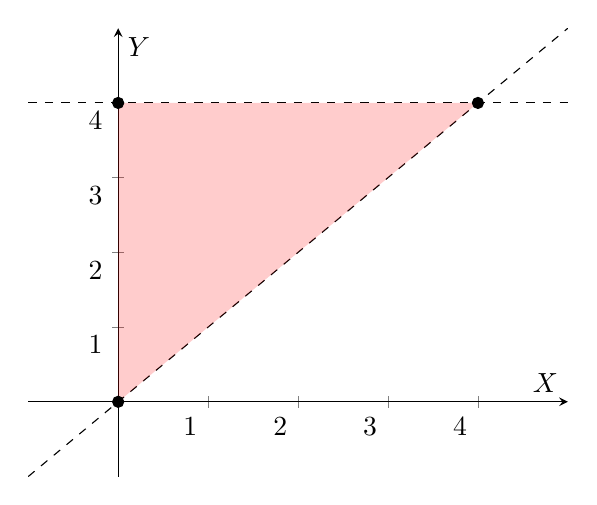
\begin{tikzpicture}
                \begin{axis}[
                    axis lines = center,
                    xlabel = $X$,
                    ylabel = $Y$,
                    xmin = -1, xmax = 5,
                    ymin = -1, ymax = 5,
                    xtick = {0,1,2,3,4},
                    ytick = {0,1,2,3,4},
                    yticklabel style = {yshift=-1.5ex},
                    xticklabel style = {xshift=-1.5ex},
                ]
                    \addplot[only marks] coordinates {
                        (0,0) (0,4) (4,4)
                    };

                    % Líneas horizontales
                    \foreach \y in {4} {
                        \addplot[dashed] coordinates {(-1, \y) (5, \y)};
                    }

                    % Representamos la recta y=x
                    \addplot[domain=-1:5, samples=2, dashed] {x};

                    % Coloreamos la región entre el (0,0), (0,4), (4,4)
                    \fill[red, opacity=0.2] (0,0) -- (0,4) -- (4,4) -- cycle;
                \end{axis}
            \end{tikzpicture}
        \end{figure}

        

        \item Probabilidad de que en una semana se venda más de la tercera parte de los litros de que se dispone al comienzo de la misma.
        \item Si en una semana se han vendido 3.000 litros de gasóleo, ¿cuál es la probabilidad de que al comienzo de la semana hubiese entre 3.500 y 3.750 litros de combustible?
    \end{enumerate}
\end{ejercicio}

\begin{ejercicio}
    Sea $(X,Y)$ un vector aleatorio continuo con función de densidad
    \[
        f(x, y) = k, \quad (x, y) \in R,
    \]
    siendo $R$ el rombo de vértices $(3,0)$; $(0,2)$; $(-3,0)$; $(0,-2)$. Calcular $k$ para que $f$ sea una función de densidad. Hallar las distribuciones marginales y condicionadas.
\end{ejercicio}

\begin{ejercicio}
    Sea $(X,Y)$ un vector aleatorio continuo con función de densidad
    \[
        f(x, y) = k, \quad x^2 \leq y \leq 1,
    \]
    anulándose fuera del recinto indicado. Hallar la constante $k$ para que $f$ sea una función de densidad de probabilidad y calcular la función de distribución de probabilidad. Calcular $P(X \geq Y)$. Calcular las distribuciones marginales y condicionadas.
\end{ejercicio}

\begin{ejercicio}
    Sea la función de densidad de probabilidad
    \[
        f(x, y) = \begin{cases}
            kxy^2 + 1, & 0 < x < 1, -1 < y < 1, \\
            0, & \text{en otro caso}.
        \end{cases}
    \]
    Calcular la función de distribución de probabilidad y las marginales.
\end{ejercicio}

\begin{ejercicio}
    Sea $(X,Y)$ un vector aleatorio bidimensional continuo, con función de densidad de probabilidad
    \[
        f(x, y) = \begin{cases}
            k, & 0 < x + y < 1, |y| < 1, 0 < x < 1, \\
            0, & \text{en otro caso}.
        \end{cases}
    \]
    Hallar la constante $k$ para que $f$ sea una función de densidad de probabilidad y calcular la función de distribución de probabilidad. Calcular las distribuciones marginales y condicionadas.
\end{ejercicio}

\begin{ejercicio}
    Sea $(X,Y)$ un vector aleatorio bidimensional continuo, con distribución de probabilidad uniforme sobre el triángulo de vértices $(0,0)$; $(0,1)$; $(1,1)$. Determinar la función de densidad de probabilidad, la función de distribución de probabilidad y las distribuciones marginales y condicionadas.
\end{ejercicio}

\begin{ejercicio}
    Sea $(X,Y)$ una variable aleatoria bidimensional con distribución uniforme en el recinto
    \[
        C = \{(x, y) \in \mathbb{R}^2; x^2 + y^2 < 1; x \geq 0, y \geq 0\}.
    \]
    Calcular:
    \begin{enumerate}
        \item La función de distribución conjunta.
        \item Las funciones de densidad marginales.
        \item Las funciones de densidad condicionadas.
    \end{enumerate}
\end{ejercicio}